
\begin{frame}{Results Obtained with Fully Automated Reasoners}
\begin{changemargin}{-0.8cm}{-1.1cm}
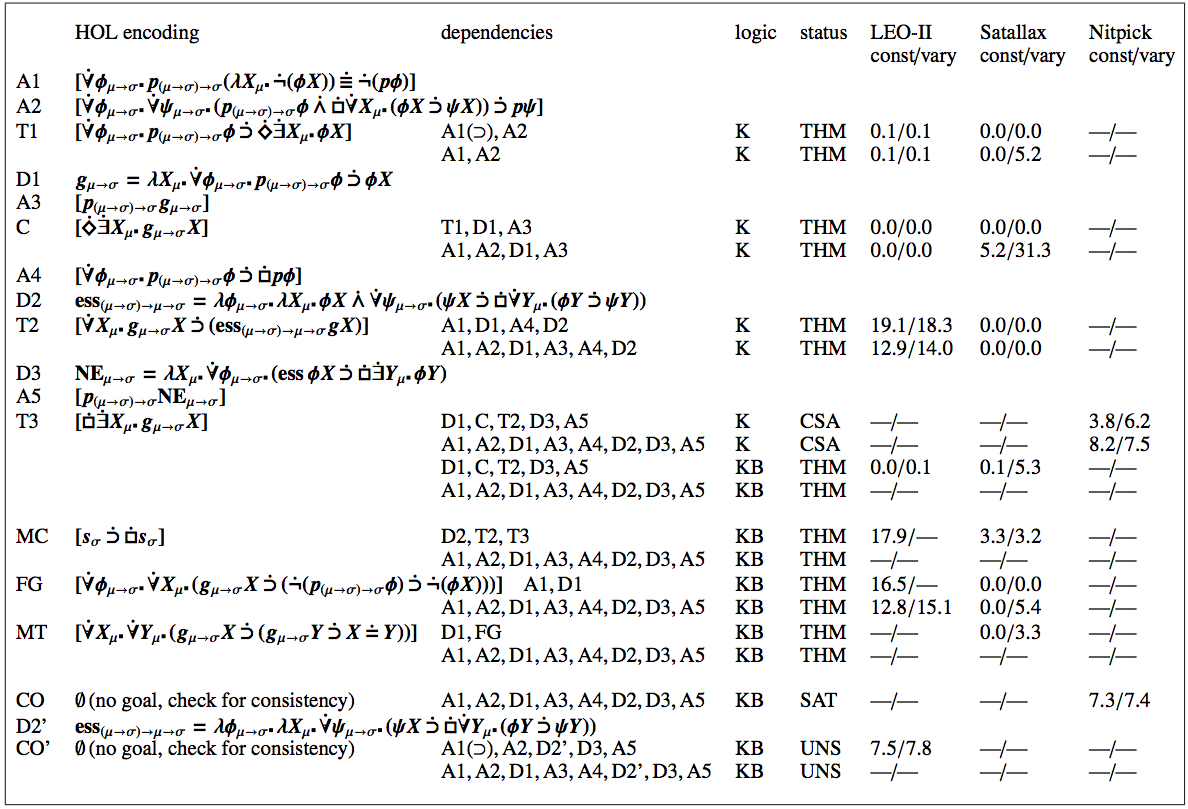
\includegraphics[width=12.4cm]{Images/Results.png}
\end{changemargin}
\end{frame}

\begin{frame}{Results Obtained with Fully Automated Reasoners}
{A controversy between Magari, H\'ajek and Anderson regarding the redundancy of some axioms}
\begin{changemargin}{-0.8cm}{-1.1cm}
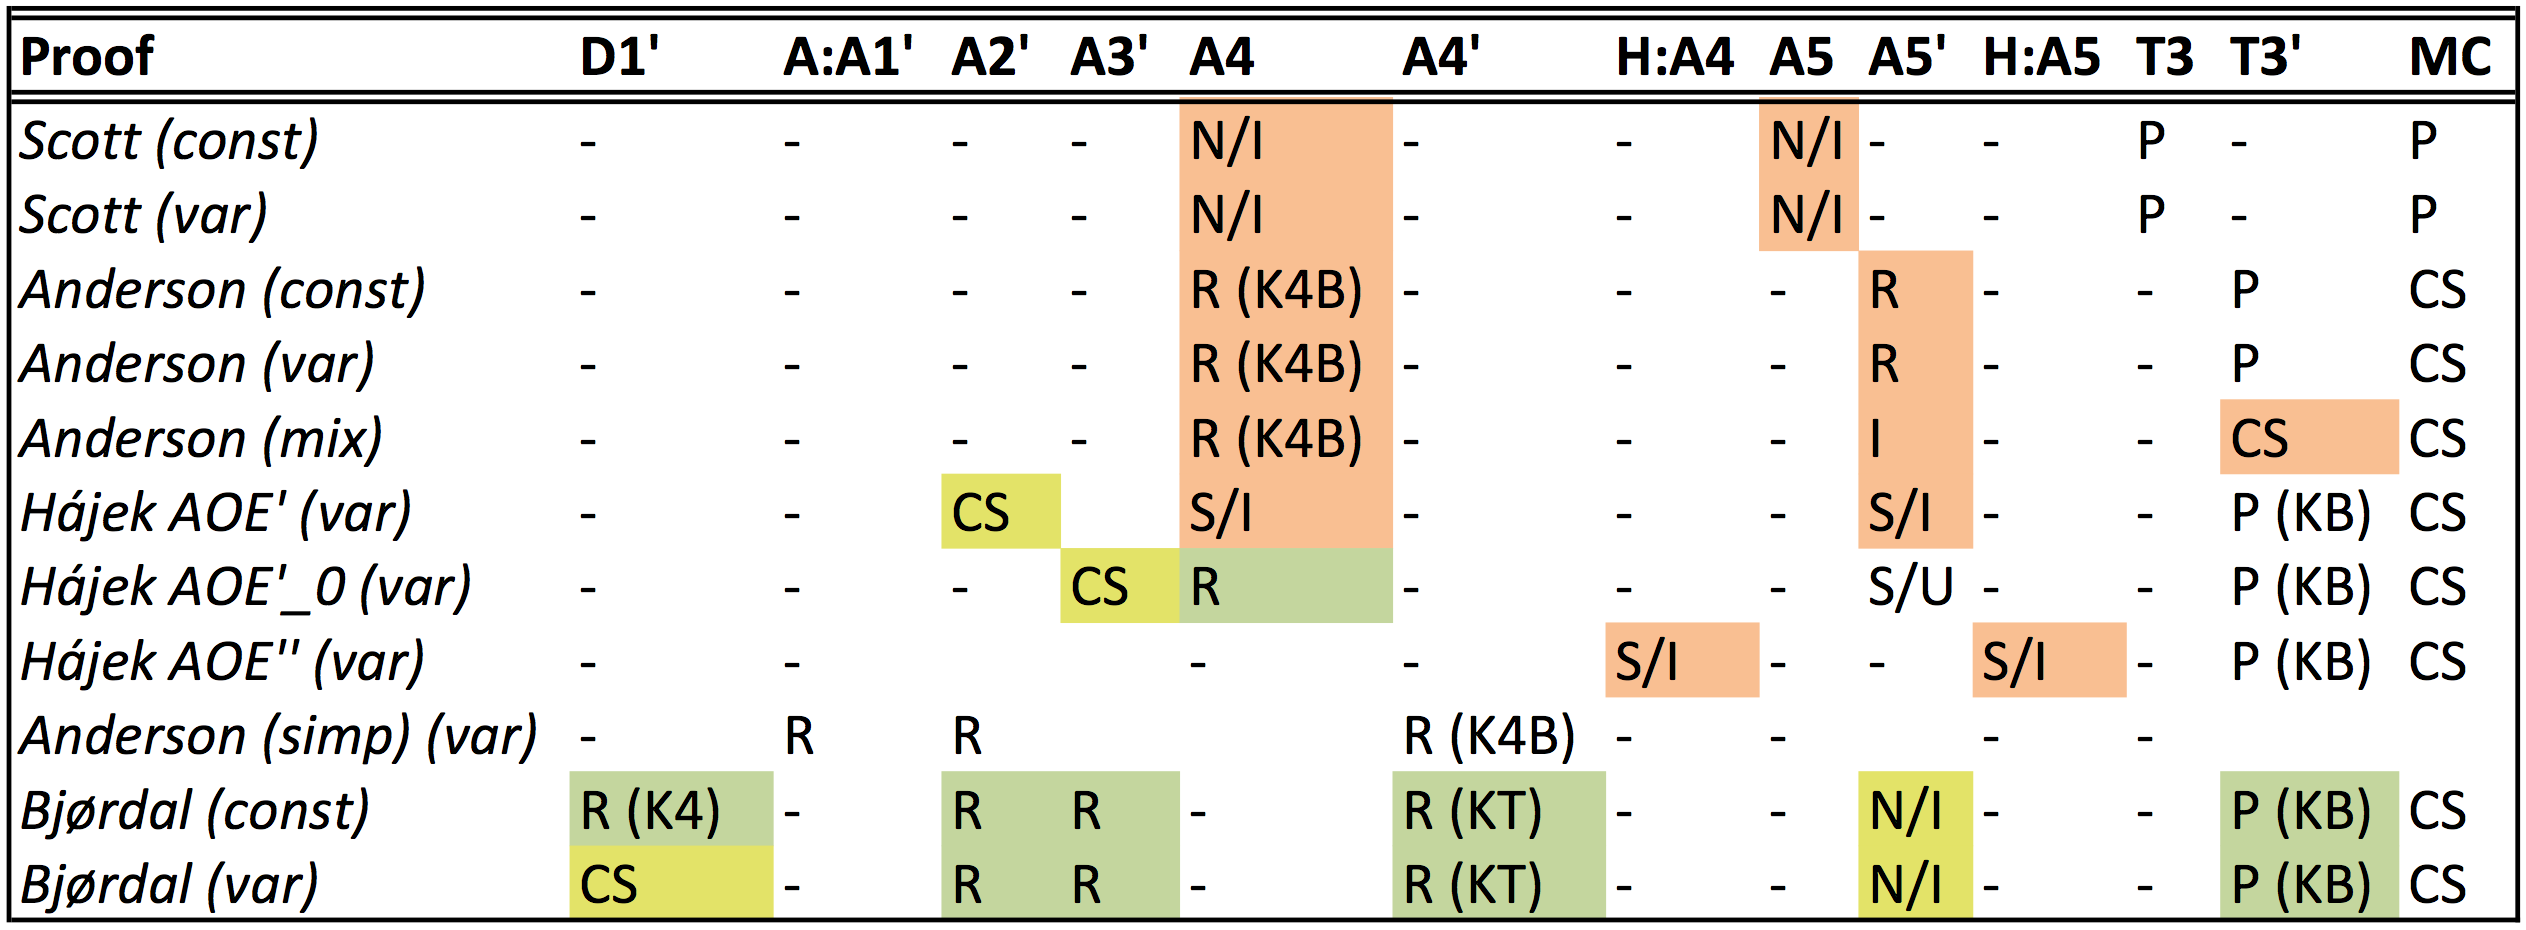
\includegraphics[width=12.4cm]{Images/ControversySummary.png}

\visible<2>{
\begin{minipage}{2.5cm}
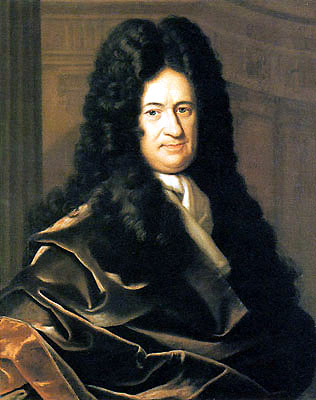
\includegraphics[width=2.5cm]{./Images/Leibniz.png} 
\end{minipage}
\begin{minipage}{9cm}
\textbf{Leibniz (1646--1716)} \\[1em]
\emph{\textbf{characteristica universalis} and  \textbf{calculus ratiocinator}} \\[0.5em]
\footnotesize
\emph{
If controversies were to arise, there would be no more need of
disputation between two philosophers than between two
accountants. For it would suffice to take their pencils in their
hands, to sit down to their slates, and to say to each other \ldots :
Let us calculate.
}
\end{minipage}
}

\end{changemargin}
\end{frame}


% \begin{frame}{The Vision of Leibniz (1646--1716): \textit{Calculemus!}}
% \begin{changemargin}{-.5cm}{-.5cm}
% \begin{minipage}{4cm}
% 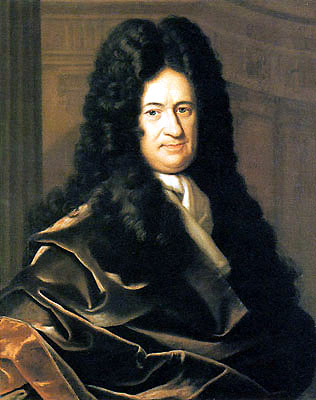
\includegraphics[width=4cm]{./Images/Leibniz.png} 

% \vspace*{1em}
% \color{gray}\footnotesize
% If controversies were to arise, there would be no more need of
% disputation between two philosophers than between two
% accountants. For it would suffice to take their pencils in their
% hands, to sit down to their slates, and to say to each other \ldots :
% Let us calculate. \\ \phantom{bla} \, \hfill (Translation by Russell)
% \end{minipage} \hfill
% \begin{minipage}{7cm} \small
% Quo facto, quando orientur controversiae, non magis disputatione opus erit inter
% duos philosophos, quam inter duos Computistas. Sufficiet enim calamos in
% manus sumere sedereque ad abacos, et sibi mutuo \ldots dicere: calculemus.
% \hfill (Leibniz, 1684)
% \vspace*{1em}

% \includegraphics[width=7cm,height=5cm]{./Images/Dispute.jpg}

% \vspace*{1em}

% \, \hfil \textbf{characteristica universalis} and  \textbf{calculus ratiocinator}
% \end{minipage}
% \end{changemargin}
% \end{frame}


\begin{frame}{Issues with Fully Automated Reasoning}{Proofs are hard to read and do not necessarily correspond to the informal proofs being verified}
\begin{changemargin}{-.5cm}{-1cm}
\colorbox{gray!20}{
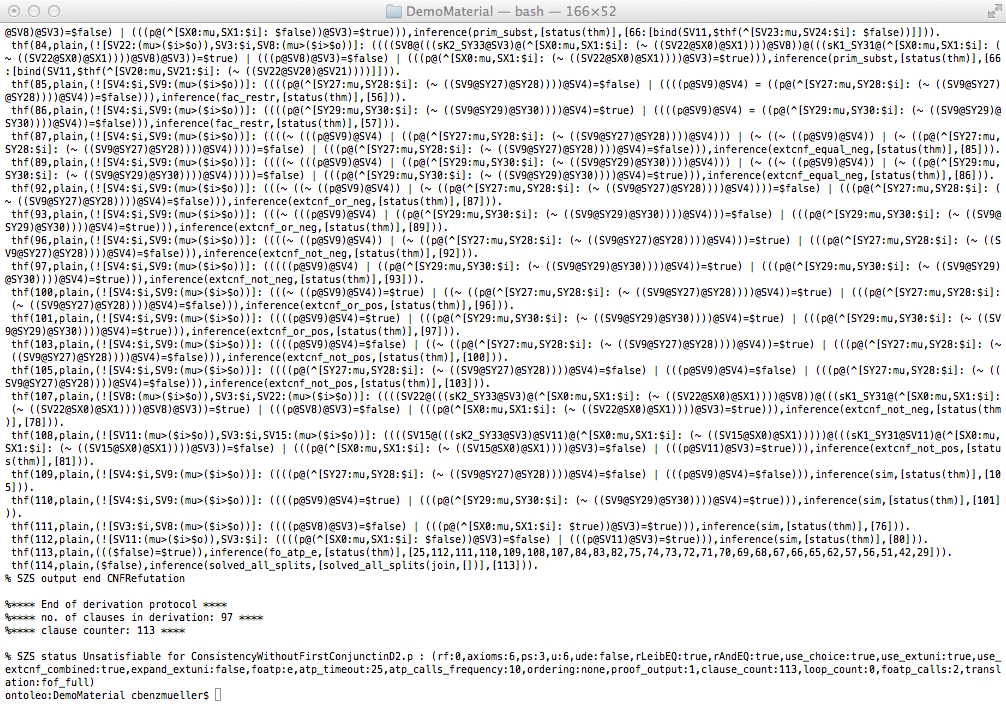
\includegraphics[width=11.5cm,height=8cm]{./Images/LeoProof.png}
}
\end{changemargin}
\end{frame}


% \begin{transitionframe}{Images/Transitions/RussianChurches}{black}
% \textbf{Formalization and Verification in Coq}
% \end{transitionframe}

\begin{frame}{The Coq Proof Assistant}
{Winner of the ACM Software System Award in 2013}
\begin{changemargin}{-1cm}{-1cm}
\colorbox{gray}{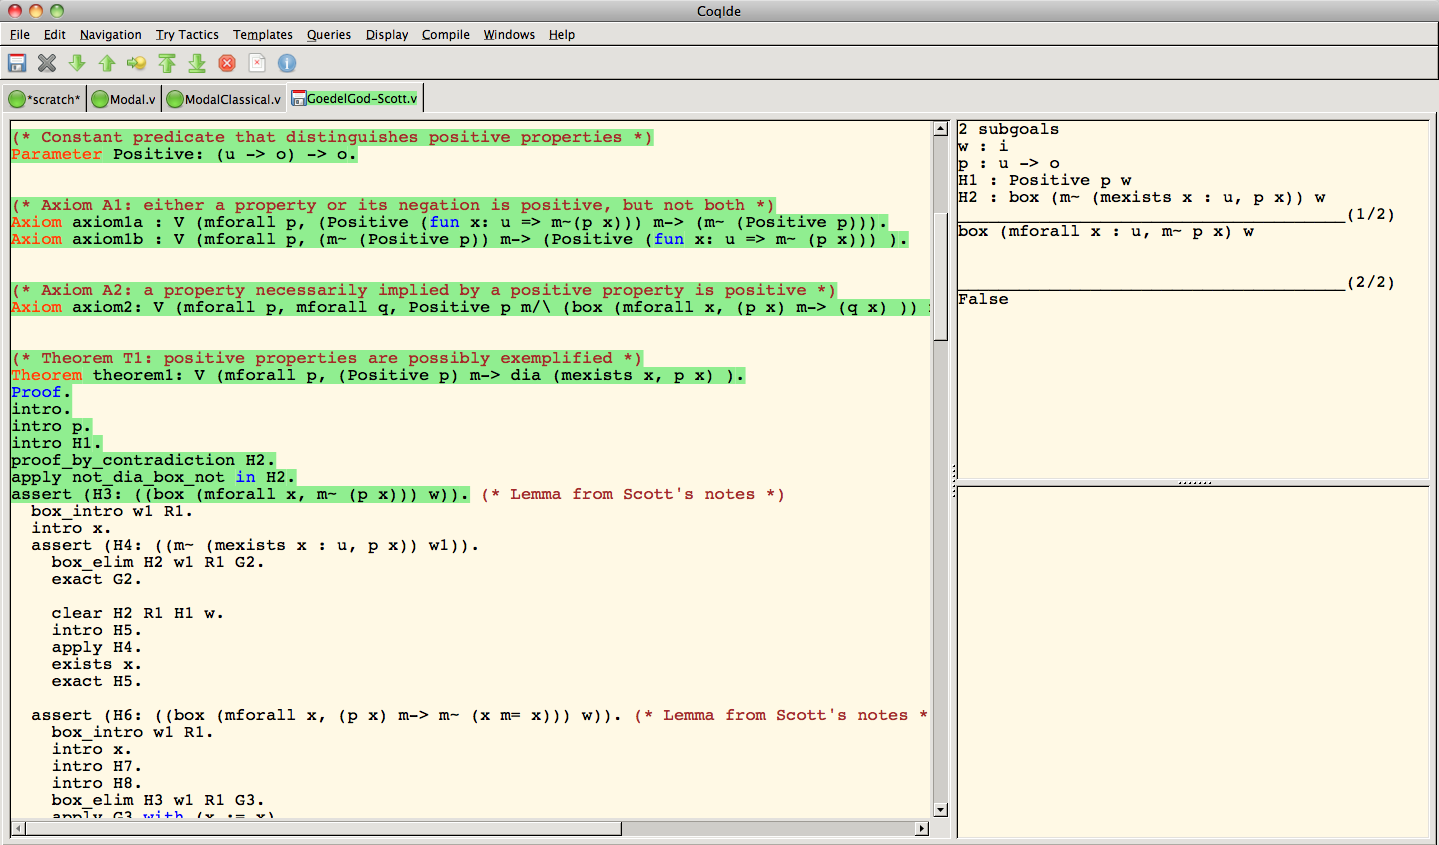
\includegraphics[width=1.17\textwidth]{Images/Demos/CoqDemo.png}}
\end{changemargin}
\end{frame}

\begin{frame}{The Proof/Type System of Coq}
\begin{itemize}
\item Calculus of Inductive Constructions (CIC)
\item Related to CC and $\lambda C$ (cf. previous talk).
\item A minimalistic higher-order natural deduction calculus.
\item Typical natural deduction rules are admissible.
\end{itemize}
\end{frame}

\begin{frame}[shrink]{Typical Natural Deduction Rules}{Interactive proving using basic tactics in Coq feels roughly like constructing a natural deduction proof}

\begin{unnamedCalculus}

\vspace{1em}

\s\s
\infer[\vee_E]{C}{A \vee B & \infer*{C}{\infer{A}{}} & \infer*{C}{\infer{B}{}}}
\s\s
\infer[\wedge_I]{A \wedge B}{A & B}
\s\s
\infer[\imp_I^h]{A \imp B}{ \infer*{B}{\infer[h]{A}{}} }

\vspace{2em}

\s\s
\infer[\vee_{I_1}]{A \vee B}{A}
\s\s
\infer[\wedge_{E_1}]{A}{A \wedge B}
\s\s
\infer[\imp_I]{A \imp B}{ B }

\vspace{2em}

\s\s
\infer[\vee_{I_2}]{A \vee B}{B}
\s\s
\infer[\wedge_{E_2}]{B}{A \wedge B}
\s\s
\infer[\imp_E]{B}{A & A \imp B}

\vspace{2em}

\s
\infer[\all_I]{\all x. A[x]}{ A[\alpha] }
\s
\infer[\all_E]{A[t]}{ \all x. A[x] }
\s\s
\infer[\ex_I]{\ex x. A[x]}{ A[t] }
\s
\infer[\ex_E]{A[\beta]}{ \ex x. A[x] }

\vspace{1em}

\s\s\s\s
$\neg A \equiv A \imp \bot$ 
\s\s\s 
\alert{\infer[\neg\neg_E]{A}{\neg\neg A}}

\vspace{1em}

\end{unnamedCalculus}

\end{frame}


\begin{frame}{Modal Logics in the Coq Proof Assistant}
\begin{itemize}
\item \begin{LARGE} Challenges: \end{LARGE} \\[0.7em]
\begin{itemize}
\item \begin{large} Can we hide the semantic embedding from the user? \end{large}\\[0.5em]
\pause
\item \begin{large} Can we provide an interaction experience to the user that differs as little as possible from what he is already used to? \end{large}\\[0.5em]
\pause
\item \begin{large} Can we reconstruct, step-by-step in Coq, precisely Scott's formulation of G\"odel's argument?  \end{large}\\[0.5em]
\end{itemize}
\end{itemize}
\end{frame}


\begin{frame}{Modal Logics in the Coq Proof Assistant}

\includegraphics[width=\textwidth]{Images/CoqCode/1.png}\\

\includegraphics[width=\textwidth]{Images/CoqCode/2.png}\\
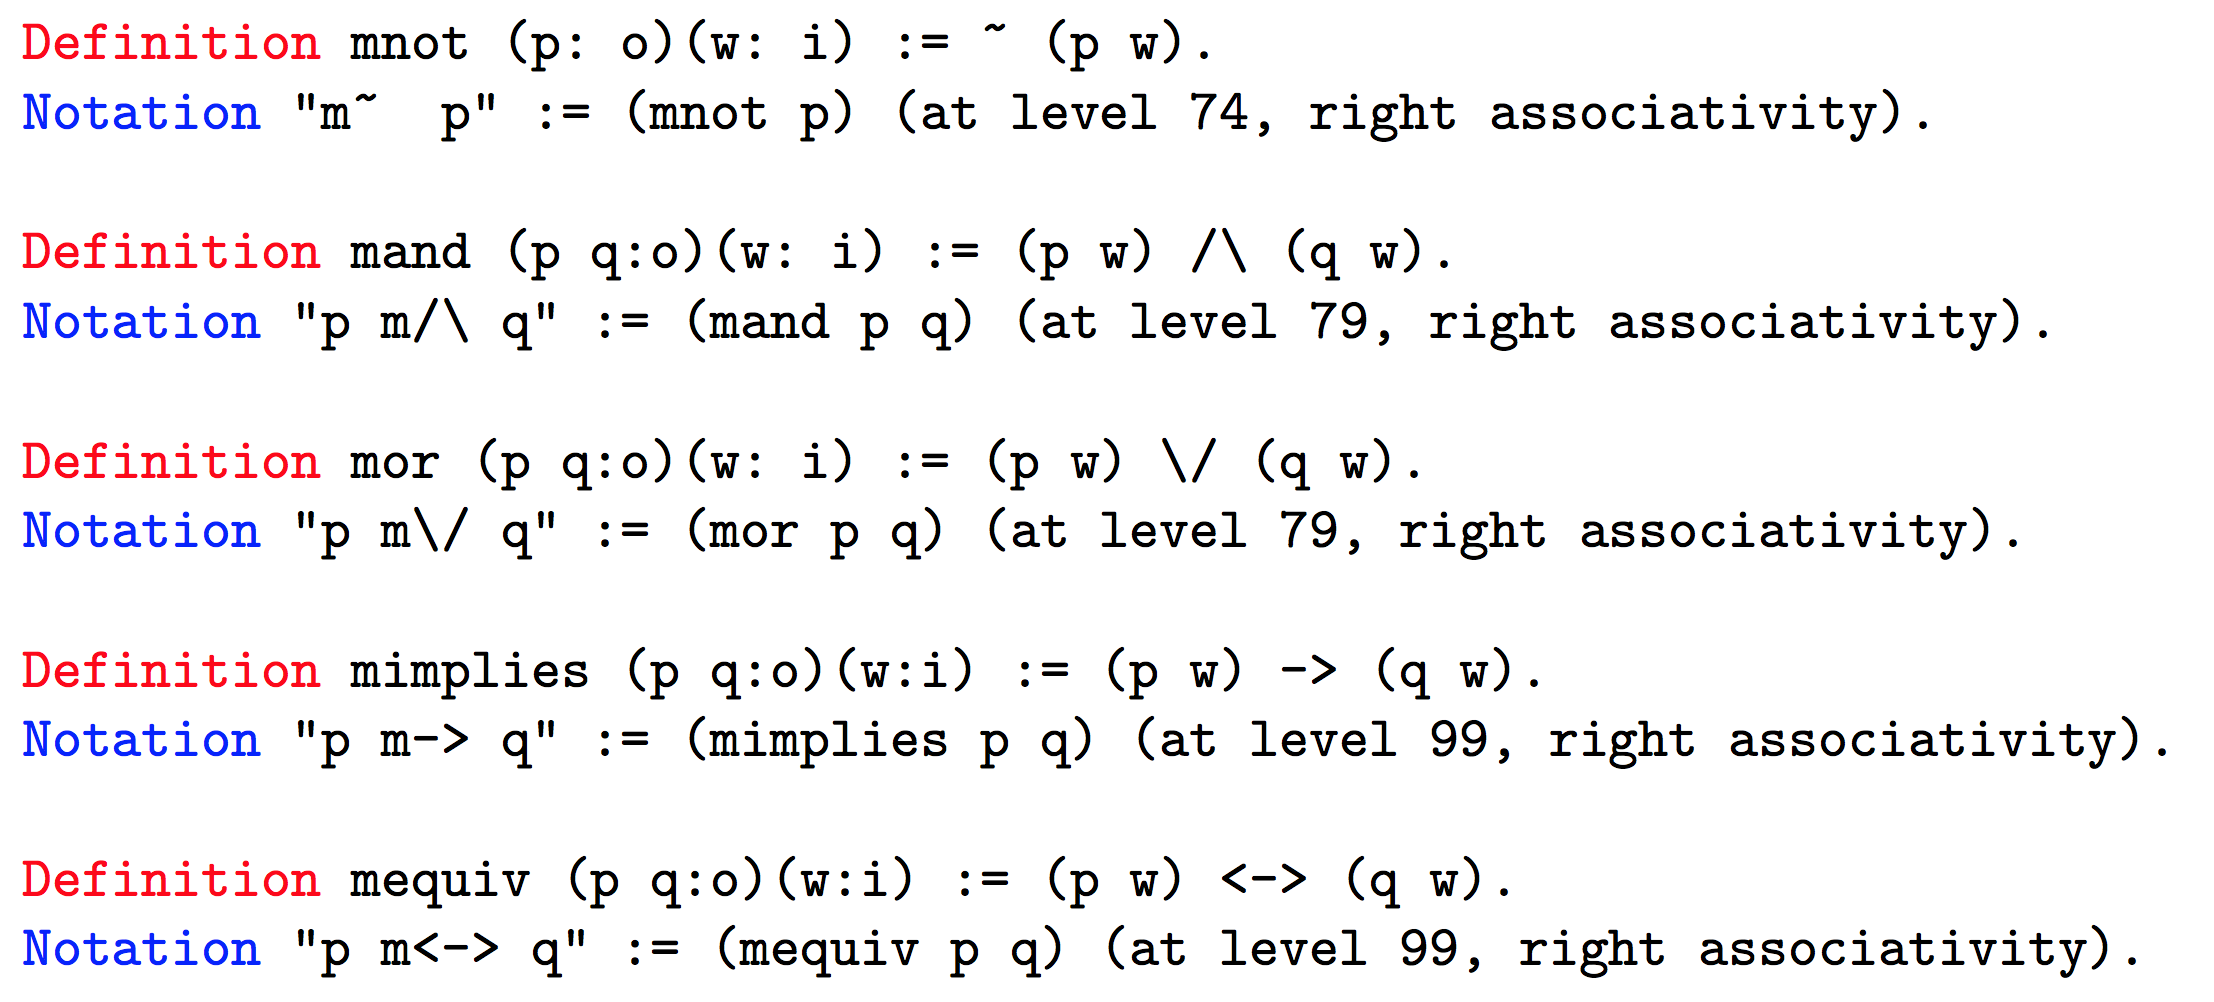
\includegraphics[width=\textwidth]{Images/CoqCode/3.png}
\end{frame}

\begin{frame}{Modal Logics in the Coq Proof Assistant}
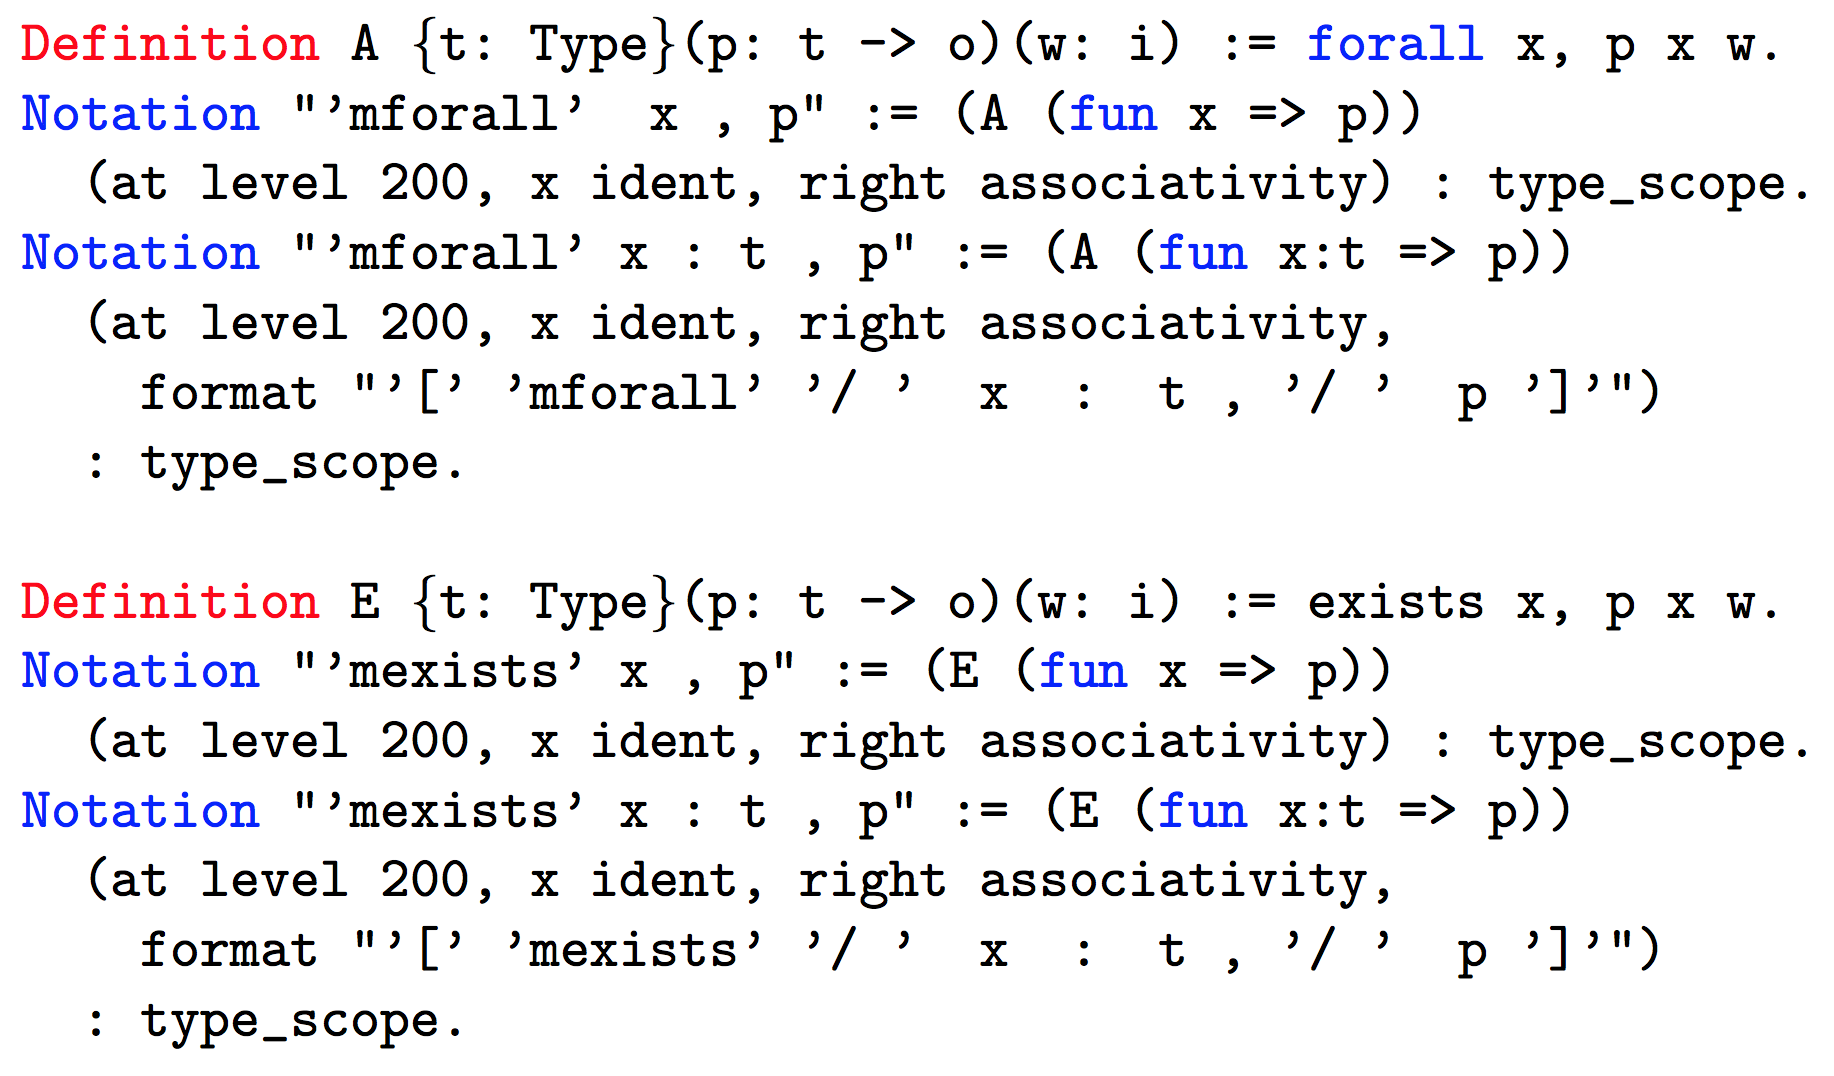
\includegraphics[width=\textwidth]{Images/CoqCode/4.png}
\end{frame}

\begin{frame}{Modal Logics in the Coq Proof Assistant}
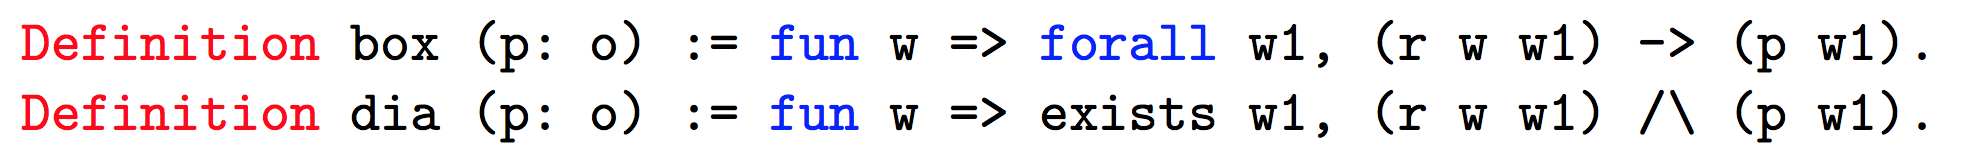
\includegraphics[width=\textwidth]{Images/CoqCode/5.png}\\
\end{frame}



\begin{frame}{Modal Logics in the Coq Proof Assistant}
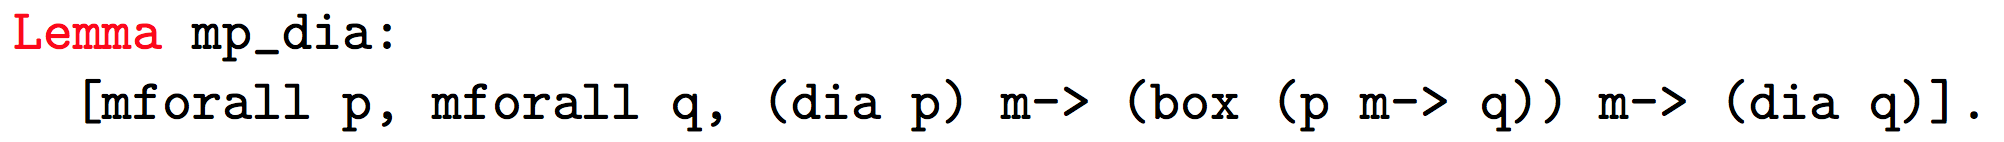
\includegraphics[width=\textwidth]{Images/CoqCode/10.png}\\
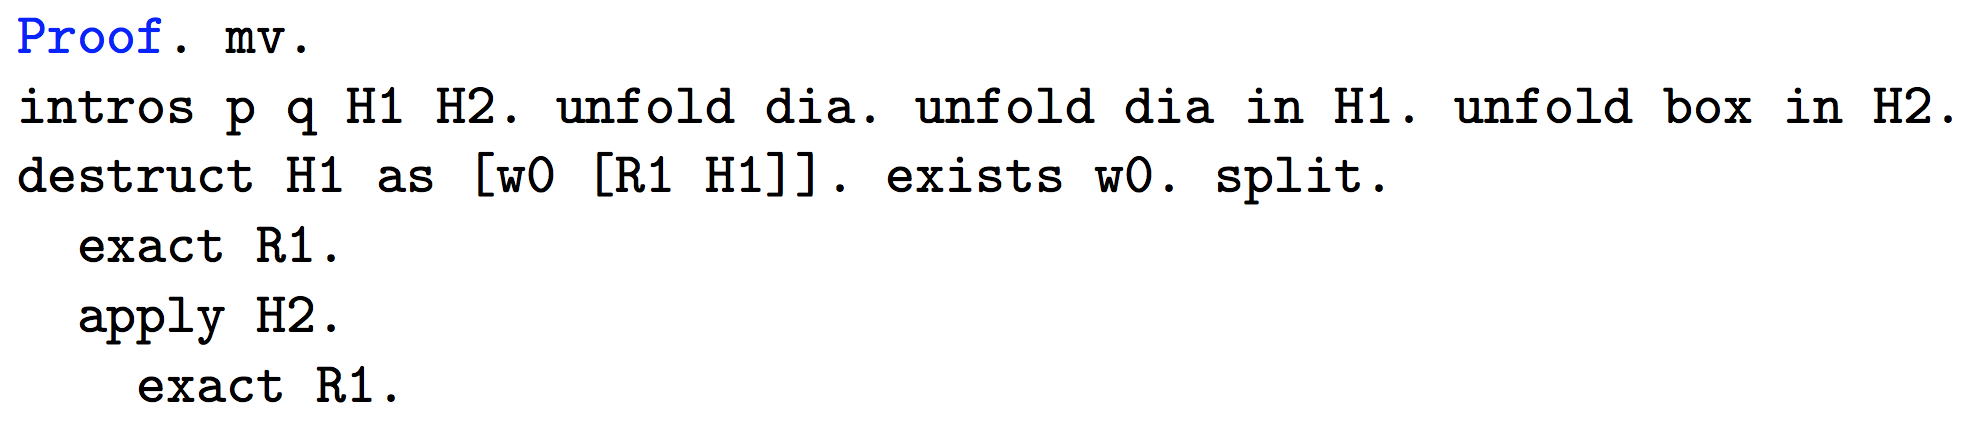
\includegraphics[width=\textwidth]{Images/CoqCode/11.png}\\
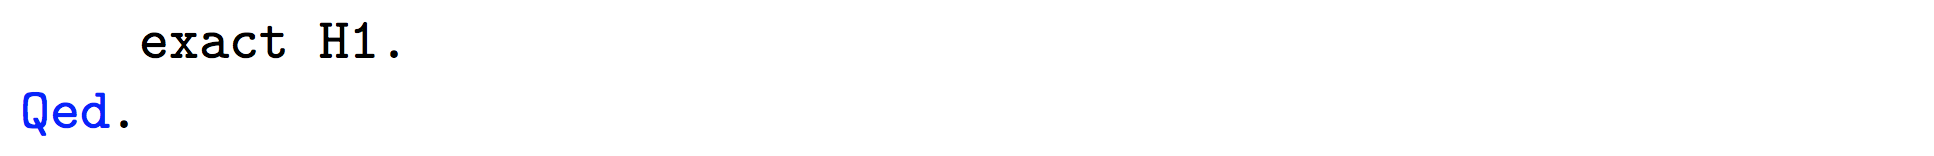
\includegraphics[width=\textwidth]{Images/CoqCode/12.png}
\end{frame}


\begin{frame}{Modal Logics in the Coq Proof Assistant}

\includegraphics[width=0.75\textwidth]{Images/CoqCode/6.png}\\
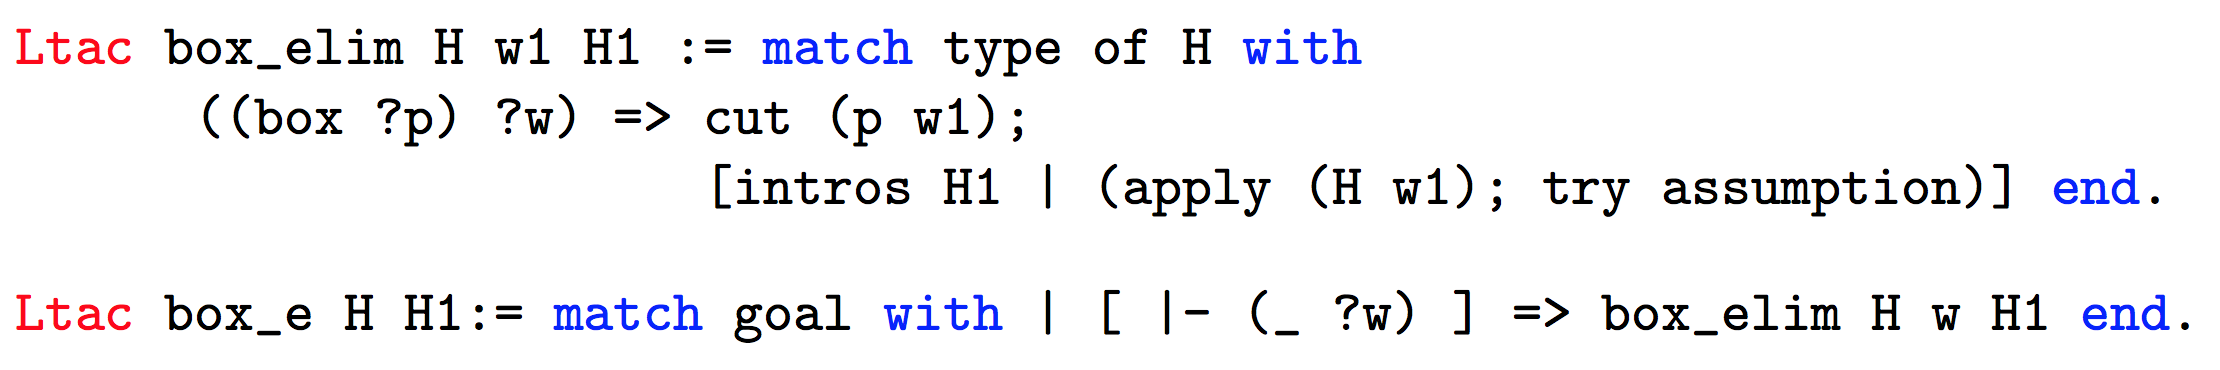
\includegraphics[width=\textwidth]{Images/CoqCode/7.png}\\

\includegraphics[width=\textwidth]{Images/CoqCode/8.png}\\

\includegraphics[width=0.8\textwidth]{Images/CoqCode/9.png}
\end{frame}

\begin{frame}{Modal Logics in the Coq Proof Assistant}
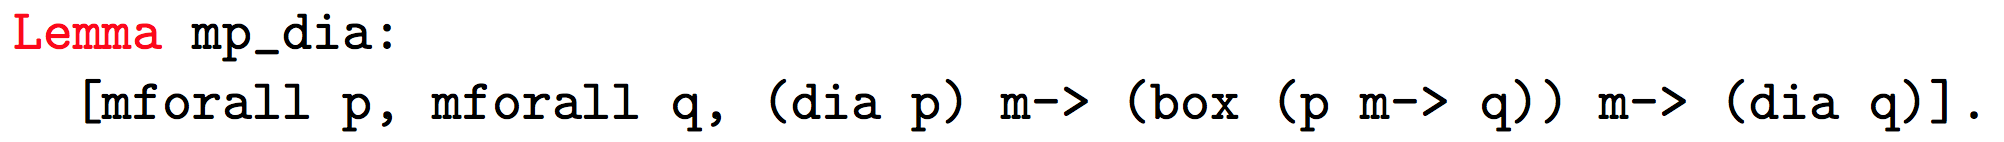
\includegraphics[width=\textwidth]{Images/CoqCode/10.png}\\
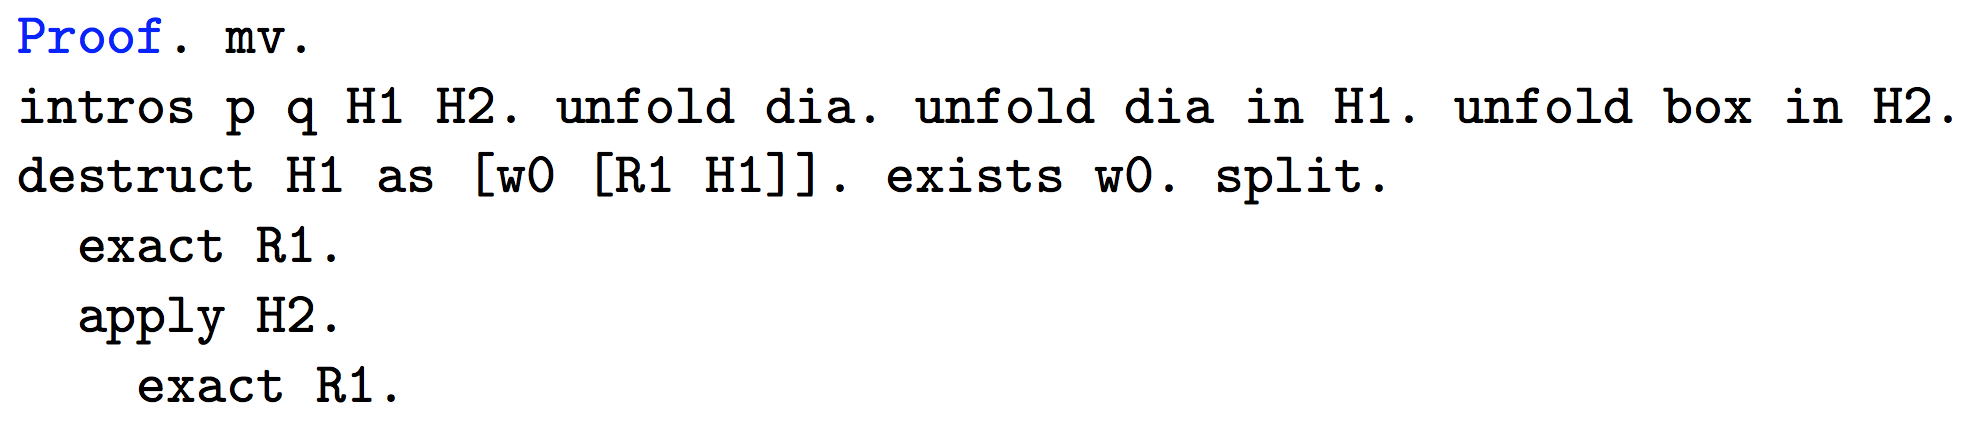
\includegraphics[width=\textwidth]{Images/CoqCode/11.png}\\
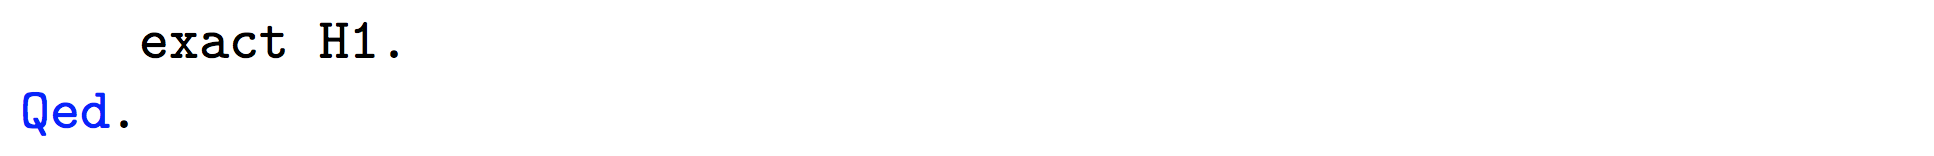
\includegraphics[width=\textwidth]{Images/CoqCode/12.png}

\bigskip

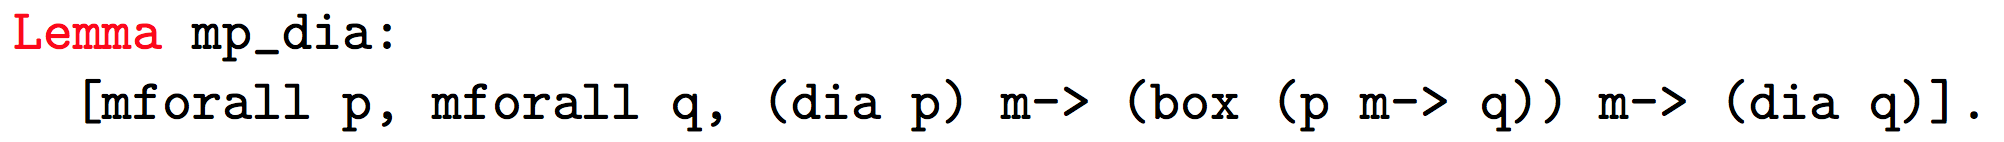
\includegraphics[width=\textwidth]{Images/CoqCode/10.png}\\
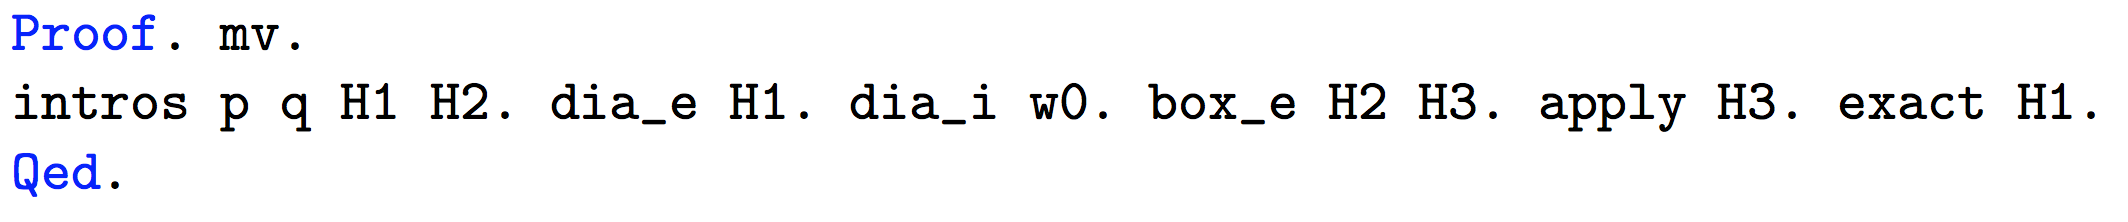
\includegraphics[width=\textwidth]{Images/CoqCode/13.png}
\end{frame}


\begin{frame}[shrink]{Natural Deduction Calculus}{Rules for Modalities}

\begin{unnamedCalculus}

\vspace{1em}

\s\s\s
\infer[\nec_I]{\nec A}{\alpha: \fbox{\infer*{A}{}} }
\s\s\s\s\s
\infer[\nec_E]{t: \fbox{ \infer*{}{A} }  }{\nec A}

\vspace{2em}

\s\s\s
\infer[\pos_I]{\pos A}{t: \fbox{\infer*{A}{}} }
\s\s\s\s\s
\infer[\pos_E]{\beta: \fbox{ \infer*{}{A} }  }{\pos A}


\vspace{1em}

\begin{center}
\textbf{eigen-box condition:}\\ 
$\nec_I$ and $\pos_E$ are \emph{strong} modal rules: \\
$\alpha$ and $\beta$ must be fresh names for the boxes they access \\ 
(in analogy to the eigen-variable condition for strong quantifier rules). \\
Every box must be accessed by \emph{exactly one} strong modal inference. \\
\vspace{0.5em}
\textbf{boxed assumption condition:} \\
assumptions should be discharged within \\
the box where they are created.
\end{center}

\end{unnamedCalculus}

\end{frame}


\begin{frame}{Modal Logics in the Coq Proof Assistant}
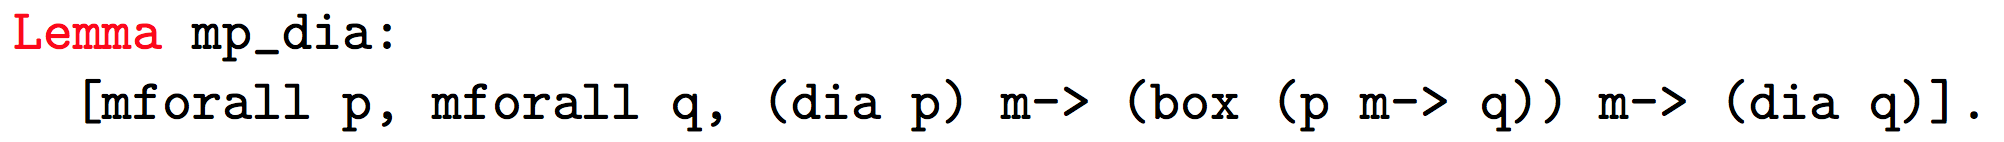
\includegraphics[width=\textwidth]{Images/CoqCode/10.png}\\
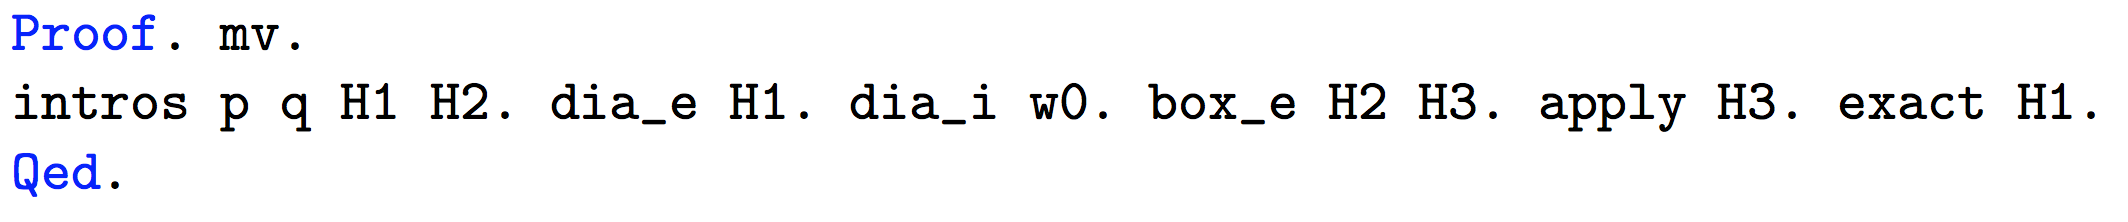
\includegraphics[width=\textwidth]{Images/CoqCode/13.png}

\bigskip

\begin{center}
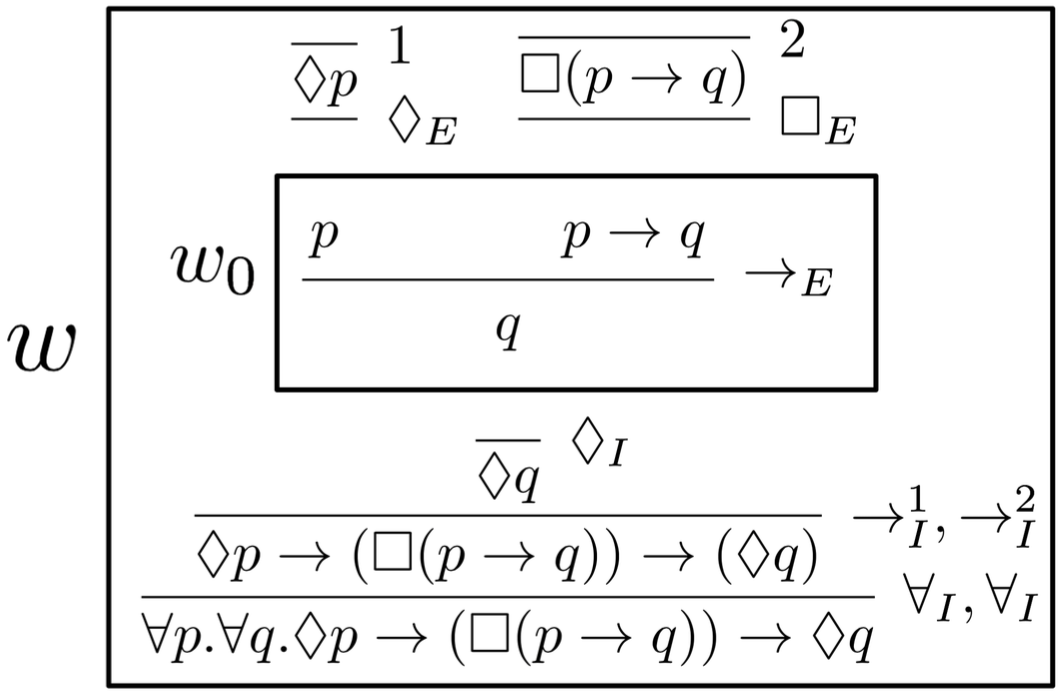
\includegraphics[width=0.8\textwidth]{Images/CoqCode/MP_Dia.png}
\end{center}

\end{frame}


\begin{frame}{Modal Logics in the Coq Proof Assistant}{Part of Scott's Formulation of G\"odel's Proof}
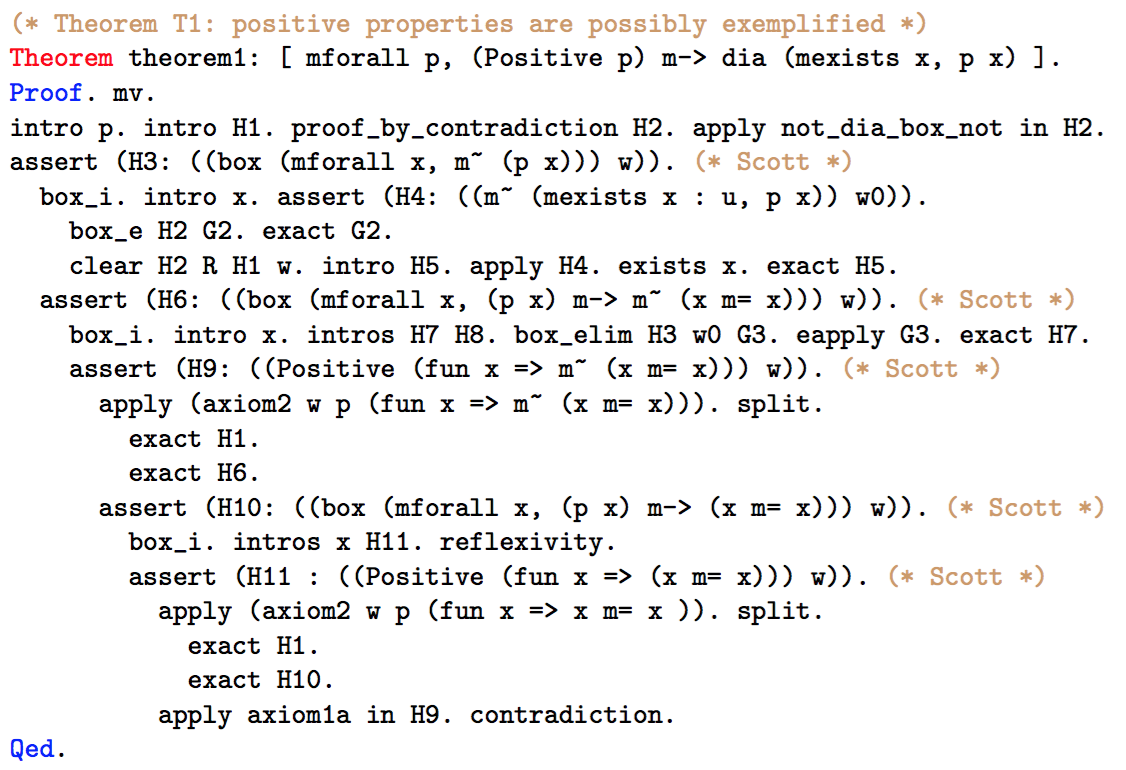
\includegraphics[width=\textwidth]{Images/CoqCode/14.png}
\end{frame}




% \begin{frame}[shrink]{Natural Deduction Calculus}{Three tiny examples}

% \vspace{1em}

% \infer[\imp_I]{A \imp A}{\infer[n]{A}{}}


% \infer[\imp_I]{A \imp A}{\infer[n]{A}{}}


% \vspace{1em}

% \end{frame}


% \begin{frame}{Natural Deduction Proofs}{T1 and C1}
% \begin{prooftree}
%         \AXC{\textbf{A2}} \dashedLine
%         \UIC{$ \all \varphi. \all \psi.[(P(\varphi) \wedge \nec \all x.[\varphi(x) \imp \psi(x)]) \imp P(\psi)]$} \RightLabel{$\all_E$}
%         \UIC{$ \all \psi.[(P(\rho) \wedge \nec \all x.[\rho(x) \imp \psi(x)]) \imp P(\psi)]$} \RightLabel{$\all_E$}
%         \UIC{$(P(\rho) \wedge \nec \all x.[\rho(x) \imp \neg \rho(x)]) \imp P(\neg \rho)$} \doubleLine
%         \UIC{$(P(\rho) \wedge \nec \all x.[\neg \rho(x)]) \imp P(\neg \rho)$}
%                         \AXC{\textbf{A1a}} \dashedLine
%                         \UIC{$\all \varphi.[ P(\neg \varphi) \imp \neg P(\varphi) ]$} \RightLabel{$\all_E$}
%                         \UIC{$ P(\neg \rho) \imp \neg P(\rho) $} \doubleLine
%                  \BIC{$ (P(\rho) \wedge \nec \all x.[\neg \rho(x)]) \imp \neg P(\rho) $} \doubleLine
%                  \UIC{$ P(\rho) \imp \pos \ex x.\rho(x) $} \RightLabel{$\all_I$}
%                  \UIC{\textbf{T1: }$\all \varphi.[ P(\varphi) \imp \pos \ex x.\varphi(x) ] $}
% \end{prooftree}

% \begin{prooftree}
% \AXC{\textbf{A3}} \dashedLine
% \UIC{$P(G)$}
%                  \AXC{\textbf{T1}} \dashedLine
%                  \UIC{$\all \varphi.[ P(\varphi) \imp \pos \ex x.\varphi(x) ]$} \RightLabel{$\all_E $}
%                  \UIC{$ P(G) \imp \pos \ex x.G(x) $} \RightLabel{$\imp_E$}
%     \BIC{$\pos \ex x. G(x)$}
% \end{prooftree}
% \end{frame}



% \begin{frame}{Natural Deduction Proofs}{T2 (Partial)}
% 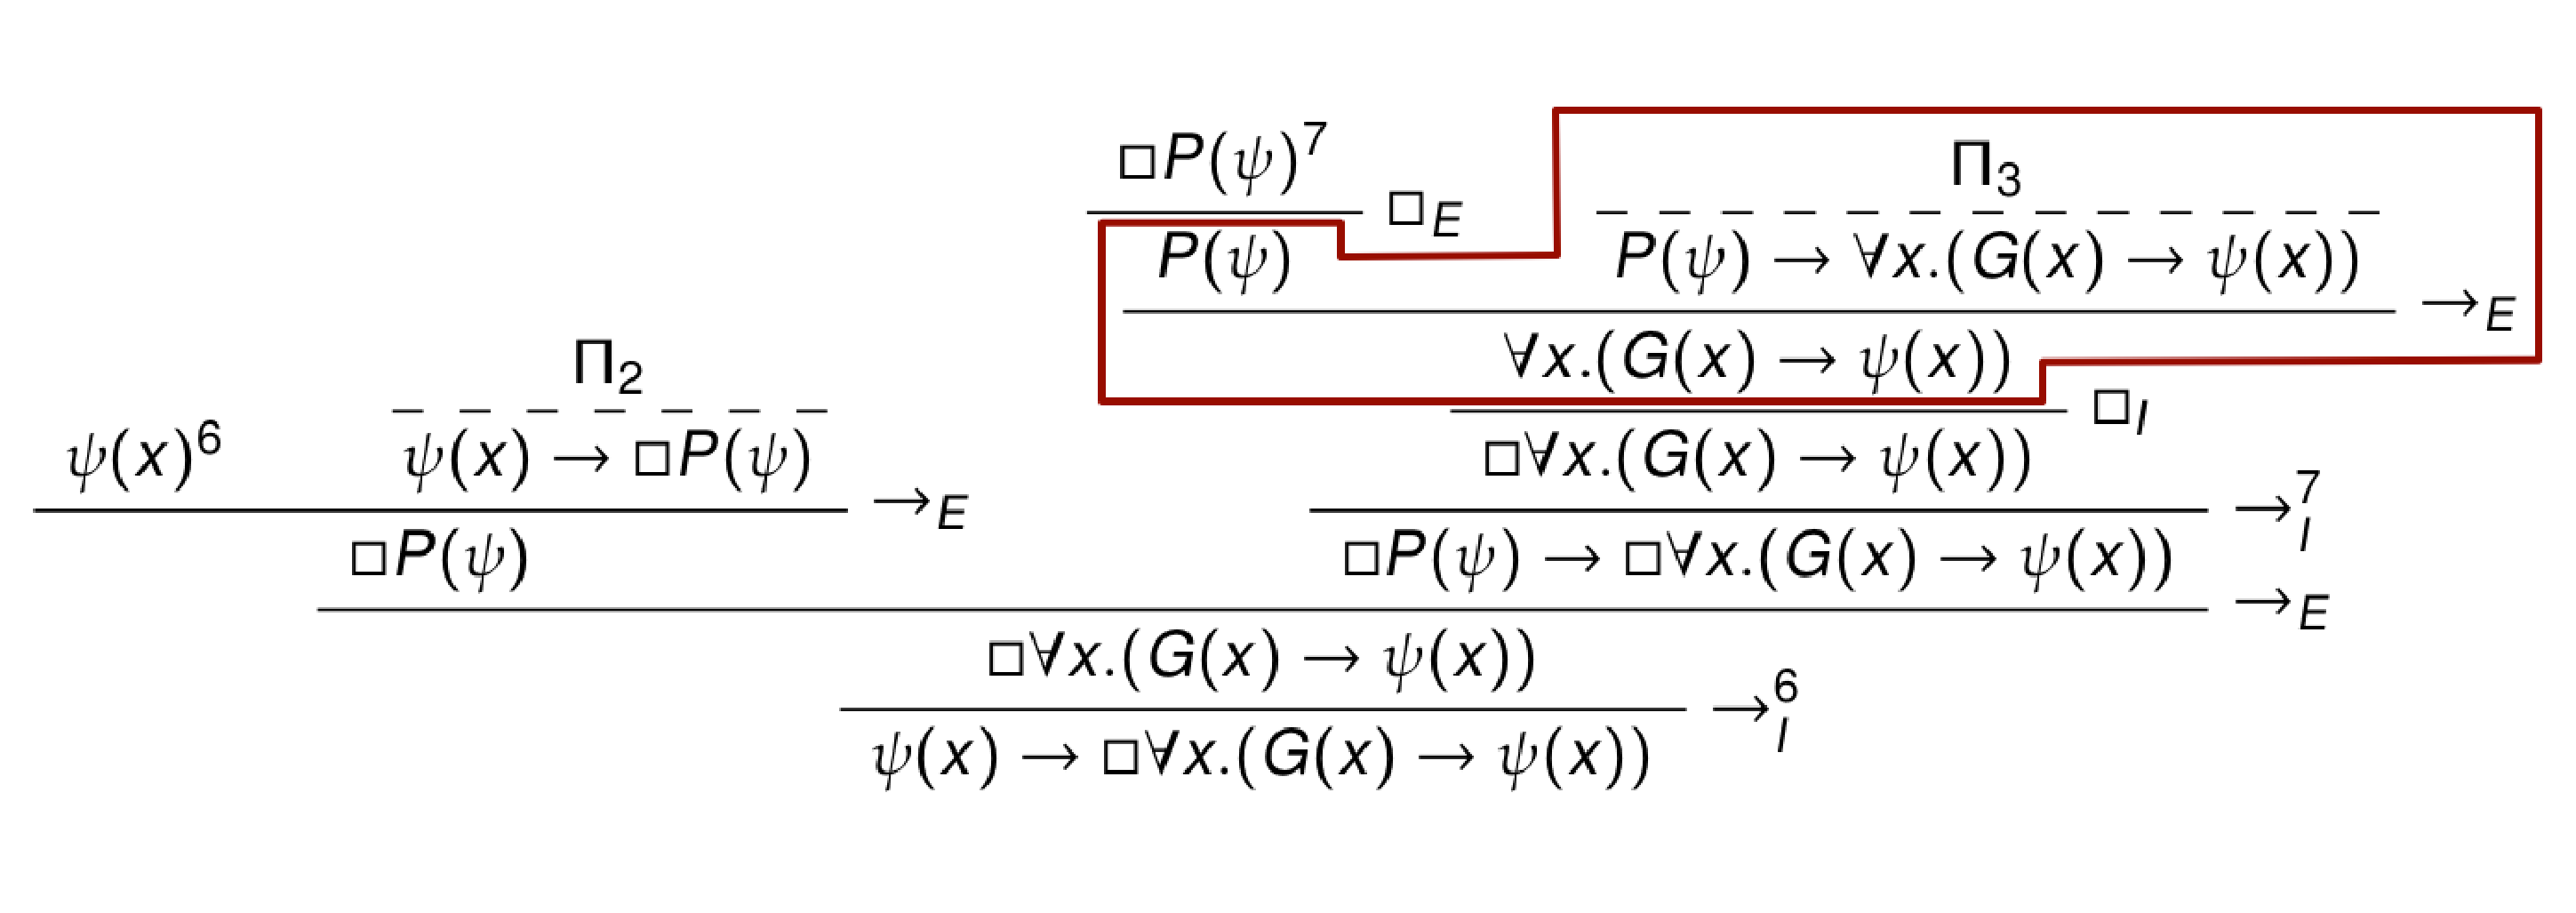
\includegraphics[scale=0.22]{Images/ProofOfT2Boxed.pdf}
% \end{frame}

